\documentclass[a4paper,4pt]{article}
\usepackage{fontspec}
\usepackage[utf8]{inputenc}
\setmainfont{Times New Roman}
\usepackage[russian]{babel}
\usepackage{geometry}
\usepackage{graphicx}
\usepackage{array}
\geometry{left=0cm,right=1cm,top=0cm,bottom=0cm}
\begin{document}
\thispagestyle{empty}
\fontsize{4pt}{4.5pt}\selectfont
% {\tiny

\begin{center}
  {\large\textbf{Шпаргалка по вычислительной математике}}
\end{center}

\vspace{0.5em}

\setlength{\extrarowheight}{2pt}
\begin{tabular}{|>{\raggedright\arraybackslash}p{0.32\textwidth}
                |>{\raggedright\arraybackslash}p{0.32\textwidth}
                |>{\raggedright\arraybackslash}p{0.32\textwidth}|} % Adjust the width of the last column
\hline
% 1-я строка, 3 ячейки
\textbf{Построение QR-разложения матрицы}
QR-разложение матрица $A$ — её представление в виде {\tiny $A = QR$}, где {\tiny $Q$} — ортогональная, {\tiny $R$} — верхняя треугольная матрица.

\textbf{Преобразования Хаусхолдера}
Исходная матрица {\tiny $A$} имеет размерность {\tiny $m \times m$}.
\begin{enumerate}
  \item {\tiny $x_1$} — первый столбец матрицы {\tiny $A$}: {\tiny $x_1 = (a_{11}, a_{21}, \dots, a_{m1})^T$}.
  Построим вектор {\tiny $v_1 = x_1 + \|x_1\|e_1$} и матрицу Хаусхолдера {\tiny $H_1$} на основе {\tiny $v_1$}. Векторы {\tiny $x_1$}, {\tiny $v_1$}, {\tiny $e_1$} имеют размерность {\tiny $m$}, а {\tiny $H_1$} — размерность {\tiny $m \times m$}.
  Ортогональная матрица {\tiny $U_1 = H_1$}. Умножим матрицу {\tiny $A$} слева на {\tiny $U_1$}. Первый столбец получившейся матрицы приобретает вид первого столбца верхней треугольной матрицы (свойство преобразования Хаусхолдера).
  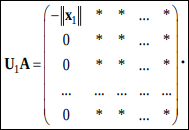
\includegraphics[width=40]{Pasted_image_20250511112728.png}
  \item Построим вектор {\tiny $x_2$} размерности {\tiny $m-1$} как второй столбец матрицы {\tiny $U_1A$} без первого элемента:
  {\tiny $x_2 = (a_{22}^*, a_{32}^*, \dots, a_{m2}^*)^T,\quad v_2 = x_2 + \|x_2\|e_1$},
  где {\tiny $e_1$} — столбец единичной матрицы {\tiny $E$} размерности {\tiny $m-1$}.
  Матрица Хаусхолдера {\tiny $H_2$} на основе {\tiny $v_2$} имеет размерность {\tiny $(m-1) \times (m-1)$}. Ортогональная матрица {\tiny $U_2$} размерности {\tiny $m \times m$}, первая строка и столбец которой совпадают с {\tiny $E$}, а остальные элементы равны {\tiny $H_2$}:

  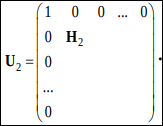
\includegraphics[width=40]{Pasted_image_20250511113950.png}

  Умножая {\tiny $U_1A$} справа на {\tiny $U_2$}, обеспечиваем два столбца верхней треугольной матрицы:

  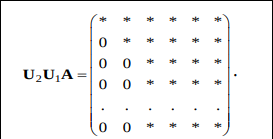
\includegraphics[width=50]{Pasted_image_20250510223317.png}
\end{enumerate}

Данный процесс позволяет получить верхнюю треугольную матрицу {\tiny $R$} за {\tiny $m-1$} шагов:

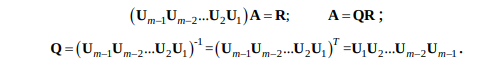
\includegraphics[width=120]{Pasted_image_20250509095614.png}

Ортогональность матрицы {\tiny $Q$} следует из симметричности и ортогональности матриц {\tiny $U_k$}.
&
\textbf{QR-алгоритм}

\textbf{Грубая схема}
Обозначим {\tiny $A_0 = A$}. На шаге с номером {\tiny $k$} выполняется
 QR-разложение матрицы {\tiny $A_k$}. Затем матрицы {\tiny $Q_k$} и {\tiny $R_k$} перемножаются в обратном порядке для получения
 {\tiny $A_{k+1}$}. При этом матрицы {\tiny $A_k$} и {\tiny $A_{k+1}$} оказываются подобными, т.е. собственные значения исходной матрицы
  в результате такого преобразования сохраняются

\textbf{Описание базового QR-алгоритма}
Для произвольной невырожденной матрицы {\tiny $A_0\in\mathbb{R}^{n\times n}$} алгоритм заключается в решениях
    {\tiny $A_k = Q_kR_k,\quad A_{k+1} = R_kQ_k$},
    где {\tiny $Q_k$} — ортогональная, а {\tiny $R_k$} — верхнетреугольная матрицы из QR-разложения {\tiny $A_k$}. Поскольку
    {\tiny $A_{k+1} = Q_k^TA_kQ_k$},
    все матрицы {\tiny $A_k$} подобны исходной, и при {\tiny $k\to\infty$} последовательность сходится к верхнетреугольному (или квазитреугольному) виду, на диагонали которого стоят собственные значения {\tiny $A_0$} .
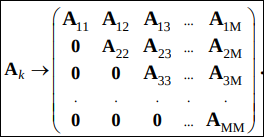
\includegraphics[width=50]{Pasted_image_20250511114857.png}
    Здесь {\tiny $A_{ii}$} квадратные подматрицы(матричные клетки), a {\tiny $A_{ij}$} = 0 для всех {\tiny i>j}

\textbf{Уменьшение числа итераций: применение сдвигов}
На каждом шаге выбирается приближение сдвига {\tiny $\tau_k$} (например, диагональный элемент {\tiny $a_{nn}^{(k)})$}, и проводят QR-разложение матрицы {\tiny $A_k - \tau_k I$}:
    {\tiny $A_k - \tau_k I = Q_kR_k,\quad A_{k+1} = R_kQ_k + \tau_k I$}.
    Такой сдвиг ускоряет сходимость к одному из собственных значений, особенно при близких корнях .
\textbf{Сокращение объёма вычислений на каждом шаге}
За счёт последовательных преобразований Хаусхолдера или Гивенса матрицу {\tiny $A_0$} приводят к верхнетреугольно-полублочному виду (Хессенберговой форме) за {\tiny $O(n^3)$}. Все последующие QR-шаги сохраняют эту форму, и один шаг QR-итерации требует {\tiny $O(n^2)$} операций вместо {\tiny $O(n^3)$} .
	Пусть матрица {\tiny $A_0$} имеет форму Хессенберга

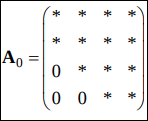
\includegraphics[width=40]{Pasted_image_20250511115916.png}

Тогда {\tiny $Q_0 = A_0R_0^{-1}$} имеет такой же вид.

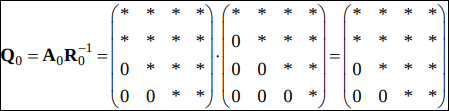
\includegraphics[width=60]{Pasted_image_20250511120006.png}

Умножая в обратном порядке убедимся, что {\tiny $A_1$} сохраняет форму {\tiny $A_0$}

  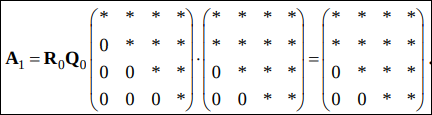
\includegraphics[width=60]{Pasted_image_20250511120043.png}


&
\textbf{Преобразование Гивенса}

Преобразование Гивенса называется преобразованием с матрицей (1) (матрицей вращения). Эта матрица отличается от единичной четырьмя элементами, стоящими на пересечении двух строк и столбцов {\tiny $k$} и {\tiny $j$}:
{\tiny $t_{kk} = t_{jj} = c, \quad t_{jk} = -t_{kj} = s, \quad c^2 + s^2 = 1.$}
Перемножая, можно понять, что матрица ортогональна:
{\tiny $T_{kj}^{-1} = T_{kj}^{T}, \quad T_{kj}^{T} \cdot T_{kj} = E.$}

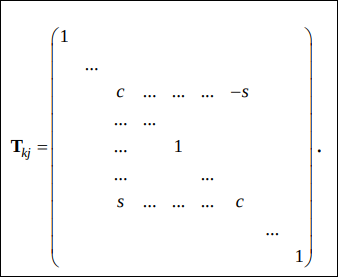
\includegraphics[width=60]{Pasted_image_20250511105511.png} (1)

Действия:
\begin{enumerate}
  \item Пусть {\tiny $A_{(k)}$} — {\tiny $k$}-й столбец {\tiny $A$}, {\tiny $A^{(k)}$} — {\tiny $k$}-я строка матрицы. Умножим {\tiny $A$} на {\tiny $T_{kj}$} ({\tiny $B = A T_{kj}$}). Матрицы {\tiny $A$} и {\tiny $B$} отличаются двумя столбцами:
  {\tiny $B_{(k)} = c A_{(k)} + s A_{(j)}, \quad B_{(j)} = -s A_{(k)} + c A_{(j)}.$}
  \item Матрицу {\tiny $T_{kj}^T$} умножим на {\tiny $B$} ({\tiny $G = T_{kj}^T B$}). Матрицы {\tiny $G$} и {\tiny $B$} отличаются двумя строками:
  {\tiny $G^{(k)} = c B^{(k)} + s B^{(j)}, \quad G^{(j)} = -s B^{(k)} + c B^{(j)}.$}
  Обозначим элементы матрицы {\tiny $G$} как {\tiny $g_{ps}$}. Для {\tiny $1 < j < k$} выберем {\tiny $s$} и {\tiny $c$} так, чтобы {\tiny $g_{k,j-1} = 0$}:
  {\tiny $g_{k,j-1} = c b_{k,j-1} + s b_{j,j-1} = c a_{k,j-1} + s a_{j,j-1}.$}
  \item Столбец {\tiny $(j-1)$} в {\tiny $A$} и {\tiny $B$} один и тот же. Выполняя {\tiny $g_{k,j-1} = 0$}, получаем следующее:
  {\tiny $\frac{s}{c} = -\frac{a_{k,j-1}}{a_{j,j-1}},$}
  {\tiny $c = \frac{a_{j,j-1}}{\sqrt{a_{k,j-1}^2 + a_{j,j-1}^2}}, \quad s = -\frac{a_{k,j-1}}{\sqrt{a_{j,j-1}^2 + a_{k,j-1}^2}}.$}
\end{enumerate}
Последовательное применение таких вращений приводит матрицу к форме Хессенберга.
\\\hline
% 2-я строка, ячейки 4–6
\textbf{Сингулярное разложение матрицы.}

Сингулярным разложением матрицы {\tiny $A\in\mathbb{R}^{m\times n}$} с вещественными элементами называется ее представление в виде
{\tiny $A = U\sum V^T \quad UU^T=E_m \quad VV^T=E_n$}
{\tiny U}-ортогональная матрица ({\tiny $m\times m$}) {\tiny V}-ортогональная матрица ({\tiny $n\times n$}), {\tiny $\sum$} - диагональная матрица ({\tiny $m\times n$}) с элементами {\tiny $\sigma_{kj} = 0$} при {\tiny $k\neq j$}

 1. Определение сингулярного разложения (SVD)

Для произвольной вещественной матрицы {\tiny $( A \in \mathbb{R}^{m \times n} )$}, сингулярное разложение имеет вид:
{\tiny $A = U \Sigma V^T,$}

где:
- {\tiny ( $U \in \mathbb{R}^{m \times m}$)}, {\tiny ( $V \in \mathbb{R}^{n \times n}$ )} — ортогональные матрицы;
- {\tiny ( $\Sigma \in \mathbb{R}^{m \times n}$ )} — диагональная матрица с неотрицательными элементами {\tiny \( $\sigma_k$ \)} на диагонали;
- {\tiny \( $\sigma_k \geq 0$ \)} — сингулярные числа матрицы {\tiny \( A \)}.
 2. Связь сингулярных чисел с {\tiny \( $A^TA$ \)} и {\tiny \( $AA^T$ \)}

Рассматриваются две симметричные матрицы:
- {\tiny \( $A^TA = V \Sigma^T \Sigma V^T$ \)},
- {\tiny \( $AA^T = U \Sigma \Sigma^T U^T$ \)}.

Таким образом, собственные значения этих матриц равны квадратам сингулярных чисел {\tiny \( $\sigma_k^2$ \)}. Если {\tiny \( $m \geq n$ \)}, то {\tiny \( $A^TA$ \)} имеет {\tiny $n$} ненулевых собственных значений (равных {\tiny \( $\sigma_k^2$ \)}), а остальные — нулевые.
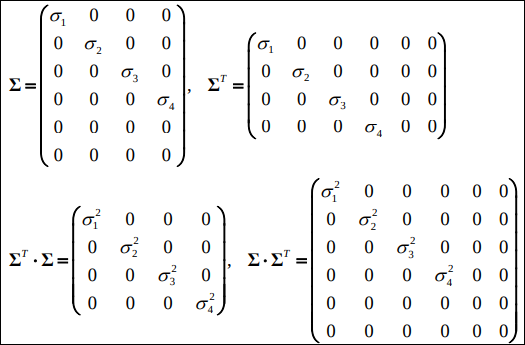
\includegraphics[width=60]{Pasted_image_20250511121951.png}
 3. Эффективный ранг и обусловленность

- Ранг матрицы равен числу ненулевых сингулярных чисел.
- Эффективный ранг — число {\tiny ( $\sigma_k$ )}, удовлетворяющих {\tiny ( $\sigma_k$ > $\varepsilon$ )}, где {\tiny ( $\varepsilon$ )} — уровень машинной точности или допустимой погрешности.
- Число обусловленности:
	{\tiny $\text{cond}(A) = \dfrac{\sigma_{\text{max}}}{\sigma_{\text{min}}}.$}
 4. Построение SVD

Реализуется двумя этапами:
1. Приведение к двухдиагональной форме с помощью преобразований Хаусхолдера.
2. QR-алгоритм для диагонализации двухдиагональной матрицы и получения {\tiny \( $\Sigma$ \)}.
 5. Программа *SVD*
Вызов:
\begin{lstlisting}
SVD(NM, M, N, A, W, MATU, U, MATV, V, IERR, RV1)
\end{lstlisting}

Параметры:
- {\tiny `A`} — исходная матрица {\tiny \( A \)};
- {\tiny `U`}, {\tiny `V`} — выходные ортогональные матрицы;
- {\tiny `W`} — сингулярные числа;
- {\tiny `IERR`} — код завершения;
- {\tiny `RV1`} — вспомогательный вектор;
- {\tiny `MATU`}, {\tiny `MATV`} — логические параметры, определяющие необходимость вычисления {\tiny `U`} и {\tiny `V`}.

 6. Применение в методе наименьших квадратов

При решении {\tiny \( $Ac \approx f$ \)}, заменяют {\tiny \( $A$ \)} на {\tiny \( $U\Sigma V^T$ \)} и получают:

{\tiny $\Sigma c' \approx f',\quad \text{где } c' = V^T c,\; f' = U^T f.$}

Задача сводится к решению:
- {\tiny \( $\sigma_k c'_k = f'_k$ \)} — если {\tiny \( $\sigma_k \neq 0$ \)},
- {\tiny \( $f'_k \approx 0$ \)} — если {\tiny \( $\sigma_k = 0$ \)}.

Решение даётся в виде:
{\tiny $c_{\text{opt}} = \sum_{k=1}^r \dfrac{f'_k}{\sigma_k} v_k,$}
где {\tiny \( $v_k$ \)} — столбцы матрицы {\tiny \( $V$ \)}, а {\tiny \( $r$ \)} — эффективный ранг.
 7. Повышение устойчивости

Если {\tiny \( $\sigma_k < \varepsilon$ \)}, соответствующие члены опускаются, уменьшая чувствительность решения к шуму в данных. Это повышает стабильность, но увеличивает невязку {\tiny \( $\|Ac - f\|$ \)}.
&
\textbf{Использование сингулярного разложения матрицы}

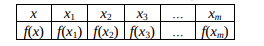
\includegraphics[width=70]{Pasted_image_20250509123644.png}
\textbf{Аппроксимация $f$:}
\tiny $Q_{n-1}(x) = c_1\varphi_1(x) + c_2\varphi_2(x) + \dots + c_n\varphi_n(x) = \sum_{k=1}^n c_k\varphi_k(x) (\tag{1})$

Коэффициенты $c_k$ определяются из условия минимума квадрата расстояния между $Q_{n-1}(x)$ и $f(x)$:
\tiny $\rho^2 = (Q_{n-1}(x) - f(x), Q_{n-1}(x) - f(x)) (\tag{2})$
Необходимое условие экстремума:
\tiny $\frac{\delta \rho^2(c_k)}{\delta c_k} = 0, \quad k = 1, 2, \dots, n$
приводит к системе линейных алгебраических уравнений, которая с ростом числа искомых коэффициентов становится катастрофически плохо обусловленной. Более надежно сингулярное разложение матрицы. Попытка максимально удачно описать табличную функцию с помощью $Q_{n-1}(x)$ приводит к:
\tiny $Ac \approx f, \quad c = (c_1, c_2, \dots, c_n)^T, \quad f = (f(x_1), f(x_2), \dots, f(x_m))^T$
где элементы прямоугольной $m \times n$ матрицы $A$ определяются по формулам:
\tiny $a_{ik} = \varphi_k(x_i), \quad i = 1, 2, \dots, m, \quad k = 1, 2, \dots, n$

Вектор невязки $r = Ac - f$. Минимизация его длины:
\tiny $(r, r) \to \min (\tag{0})$
полностью совпадает с задачей минимизации $\rho^2$. Будем искать $c$, чтобы квадрат длины вектора невязки был минимален. Заменяя в (3) матрицу $A$ её сингулярным разложением $U\Sigma V^T$ и умножая на $U^T$, получаем:
\tiny $\Sigma V^T c \approx U^T f \quad \Rightarrow \quad \tilde{c} = V^T c, \quad \tilde{f} = U^T f, \quad c = V \tilde{c}, \quad f = U \tilde{f} (\tag{4})$
\tiny $\Sigma \tilde{c} \approx \tilde{f} (\tag{5})$
Вектор невязки:
\tiny $\tilde{r} = \Sigma \tilde{c} - \tilde{f}$
Длина осталась прежней.

\textbf{Решение (5):}

\textbf{1 случай:} $m \geq n$

Две подсистемы:
\tiny $\tilde{c}_k \sigma_k \approx \tilde{f}_k, \quad k = 1, 2, \dots, n (\tag{6})$
\tiny $0 \approx \tilde{f}_k, \quad k = n+1, \dots, m (\tag{7})$
Сингулярные числа упорядочены по убыванию. Если $m = n$, подсистема (7) отсутствует. Минимум $\rho^2$ и условие (0) из (6) решается точно ($\sigma_k \neq 0$):
\tiny $\tilde{c}_k = \frac{\tilde{f}_k}{\sigma_k}, \quad k = 1, 2, \dots, n (\tag{8})$
\tiny $\min(\rho^2) \quad \Rightarrow \quad (r, r) = (\tilde{r}, \tilde{r}) = \sum_{k=n+1}^m \tilde{f}_k^2 (\tag{9})$

\textbf{2 случай:} $m < n$

Все сингулярные числа не нулевые, подсистема (7) отсутствует. Из (6):
\tiny $\tilde{c}_k \sigma_k = \tilde{f}_k, \quad k = 1, 2, \dots, m$
Первые $m$ значений выбираются из условия:
\tiny $\tilde{c}_k = \frac{\tilde{f}_k}{\sigma_k}, \quad k = 1, 2, \dots, m$
Остальные $\tilde{c}_k$ выбираются произвольно.
&
\textbf{Псевдообратная матрица Мура-Пенроуза}

\tiny $A^+ \text{ — псевдообратная матрица, } x = A^+b$
Если $A$ имеет полный столбцовый ранг, то:
\tiny $A^+ = (A^TA)^{-1}A^T$
\tiny $(r, r) = (Ax - b, Ax - b) = (Ax, Ax) - 2(Ax, b) + (b, b) = (A^TAx, x) - 2(x, A^Tb) + (b, b) \to \min$
Необходимое условие минимума:
\tiny $\frac{\delta(r, r)}{\delta x} = 2A^TAx - 2A^Tb = 0$
\tiny $x = (A^TA)^{-1}A^Tb = A^+b, \quad A^+ = (A^TA)^{-1}A^T$

\textbf{Псевдообратной матрицей Мура-Пенроуза} называется матрица $X = A^+$, удовлетворяющая 4 условиям:
$AXA = A$
$XAX = X$
$AX$ — симметричная
$XA$ — симметричная

Можно показать, что такая матрица $X$ существует и единственна, и для её построения применяется сингулярное разложение.

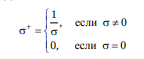
\includegraphics[width=70]{Pasted_image_20250509144613.png}

Для $A = \sigma$ (1 × 1) определить $X$ как $X = \sigma^+$ — все 4 условия выполняются.

В общем случае для $\Sigma$ (m × n):

\(\Sigma^+ \text{ (n × m) } \quad \Rightarrow \quad X = A^{+} = V\Sigma^+U^{T}\)

\[
\Sigma =
\begin{pmatrix}
  \sigma_{1} & \cdots & \cdots & 0 \\
  \vdots & \ddots & \cdots & \cdots \\
  0 & \vdots & 0 & \sigma_{N} \\
  0 & \vdots & \cdots & 0
\end{pmatrix}
\]

\[
\Sigma^{+} =
\begin{pmatrix}
  \sigma_{1}^{+} & \cdots & \cdots & 0 \\
  \vdots & \ddots & \cdots & 0 \\
  0 & \vdots & \sigma_{N}^{+} & 0
\end{pmatrix}
\]

\(\Sigma \cdot \Sigma^{+} = \Sigma \text{ но вместо } \sigma - (0) \quad \Sigma^{+} \cdot \Sigma = E \quad \Sigma \cdot \Sigma^{+} \cdot \Sigma = \Sigma \quad \Sigma^{+} \cdot \Sigma \cdot \Sigma^{+} = \Sigma^{+}\)

Последние два равенства верны и в случае, когда среди последних сингулярных чисел есть нулевые. С учётом этих равенств:
\(AXA = U\Sigma V^{T}V\Sigma^{+}U^{T}U\Sigma V^{T} = U\Sigma\Sigma^{+}\Sigma V^{T} = U\Sigma V^{T} = A\)
\(XAX = V\Sigma^{+} U^{T}U\Sigma V^{T}V\Sigma^{+} U^{T} = V\Sigma^{+}\Sigma\Sigma^{+}U^{T} = V\Sigma^{+}U^{T} = X\)

Матрицы $AX$ и $XA$ — симметрические. Для $m < n$ аналогично.

Пусть $A \to a_{ij}$, $A^+ \to A_{ij}^+$, $U \to u_{ij}$, $V \to v_{ij}$ — элементы. Тогда:
\tiny $a_{ij} = \sum_{k=1}^n \sigma_k u_{ik}v_{jk}, \quad a_{ij}^+ = \sum_{\sigma_k \neq 0} \frac{v_{ik}u_{jk}}{\sigma_k}$

\textbf{Эффективная псевдообратная матрица} $A^+_\varepsilon$ уменьшает число обусловленности, повышая надёжность результатов:

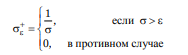
\includegraphics[width=70]{Pasted_image_20250509145757.png}
\tiny $a_{ij}^+(\varepsilon) = \sum_{\sigma_k > \varepsilon} \frac{v_{ik}u_{jk}}{\sigma_k}$

Эффективная псевдообратная матрица удовлетворяет трём последним условиям, а первое выполняется с точностью до $\varepsilon$:
\tiny $||AXA - A|| \leq \varepsilon$

Для ненулевого значения $\varepsilon$ $X$ может оказаться неединственной, удовлетворяющей этим 4 условиям. Но матрица с такими элементами дополнительно обладает наименьшей нормой.
\\\hline

% \multicolumn{3}{|p{0.90\textwidth}|}{
Любой одношаговый итерационный метод для системы $Ax = b$ можно записать в виде $B_{n+1},\frac{x_{n+1} - x_n}{\tau_{n+1}} + Ax_n = b$ где $x_n$ — текущее приближение, $x_{n+1}$ — следующее;  $B_{n+1}$ — матрица, задающая структуру метода;   $\tau_{n+1}$ — шаг (или параметр релаксации) на шаге $n+1$

По выбору $B_{n+1}$ и $\tau_{n+1}$ различают: \textbf{явные} ($B_{n+1} = E$) и \textbf{неявные} ($B_{n+1}\neq E$); \textbf{стационарные} ($B_{n+1}=\mathrm{const},,\tau_{n+1}=\mathrm{const}$) и \textbf{нестационарные} ($\tau_{n+1}$ и/или $B_{n+1}$ меняются)

D - диагональная, $A_1$ - левая треугольная, $A_2$ - левая треугольная

Примеры:

1. \textbf{Метод простой итерации}
- $B_{n+1}=E$, $\tau_{n+1}=\tau=\mathrm{const}$  Итерация: $x_{n+1} = (E - \tau A),x_n + \tau b$ Условие сходимости: $0 < \tau < \tfrac{2}{\lambda_{\max}(A)}$

2. \textbf{Итерационный метод Ричардса}
$B_{n+1}=E$, но $\tau_{n+1}$ меняется от итерации к итерации Итерация:  $x_{n+1} = x_n + \tau_{n+1}(b - A,x_n)$ Оптимальный подбор $\tau_{n+1}$ (например, на основе полиномов Чебышева) ускоряет сходимость

3. \textbf{Метод Якоби}
Разбиение $A = D + L + U$, где $D$ — диагональная часть, $L$ — нижняя треугольная, $U$ — верхняя $B_{n+1}=D$, $\tau_{n+1}=1$  Итерация:  $x_{n+1} = D^{-1}(b - (L+U),x_n)$

4. \textbf{Метод Гаусса–Зейделя}
$B_{n+1}=D + L$, $\tau_{n+1}=1$ Итерация: $x_{n+1} = -(D+L)^{-1}U,x_n + (D+L)^{-1}b$ При вычислении $x_{n+1}^{(k)}$ используются уже обновлённые $x_{n+1}^{(j)}$ для $j<k$

5. \textbf{Метод верхней релаксации}
(SOR) $B_{n+1} = D + \omega L$, $\tau_{n+1}=\omega$, где $0 < \omega < 2$ При $\omega = 1$ метод совпадает с методом Гаусса–Зейделя
&
% ...existing code...

\end{tabular}

% }


\end{document}
